\documentclass[12pt]{article}

\usepackage[utf8]{inputenc}
\usepackage[T1]{fontenc}
\usepackage{amsmath}
\usepackage{booktabs}
\usepackage{graphicx}
\usepackage{xcolor}
\usepackage{geometry}
\usepackage{hyperref}
\usepackage{natbib}
\usepackage{longtable}
\usepackage{array}
\usepackage{pdflscape}
\usepackage{float}
\usepackage[margin=10pt,font=small,labelfont=bf]{caption}

\geometry{margin=1in}
\graphicspath{{Paper/figures/}{figures/}}
\hypersetup{
  colorlinks=true,
  linkcolor=blue!55!black,
  citecolor=blue!55!black,
  urlcolor=blue!55!black
}

\title{Sectoral Sources of Total Factor Productivity Growth in Colombia, 2005--2024}
\author{
Oliver Pardo\thanks{Associate Professor, Departamento de Administraci\'on, Pontificia Universidad Javeriana; Director, Centro Javeriano de Competitividad. Corresponding author: \href{mailto:pardoo@javeriana.edu.co}{pardoo@javeriana.edu.co}.}
\and
Jorge Orozco\thanks{Research Consultant, Centro Javeriano de Competitividad, Pontificia Universidad Javeriana.}
}
\date{July 2026}

\begin{document}

\maketitle

\begin{abstract}
This paper reconstructs the long-run evolution of total factor productivity (TFP) for the Colombian economy and nine economic activities using the annual production-account results published by the national statistical office (DANE). We chain the 19 annual log changes from 2006 to 2024, recover the annual aggregation weights implicit in the publication, and decompose aggregate TFP into exact activity contributions. The aggregate TFP index fell from 100 in 2005 to 98.5 in 2024, equivalent to $-0.081$ percentage points per year. This small aggregate decline conceals large sectoral differences. Agricultural TFP increased by 27.6 percent, while mining TFP fell by 35.1 percent. Four activities contributed 0.361 percentage points per year to aggregate TFP, but five activities subtracted 0.441 points. An accounting counterfactual that sets annual TFP growth to zero in mining, construction, finance and real estate, and manufacturing raises production-account output growth from 3.15 to 3.59 percent per year. The exercise measures an accounting margin, not a causal policy effect or a counterfactual path for GDP.
\end{abstract}

\noindent\textbf{Keywords:} total factor productivity; growth accounting; KLEMS; sectoral productivity; Colombia.

\noindent\textbf{JEL codes:} O47; O54; E23; C43.

\section{Introduction}

Colombia's near-zero aggregate total factor productivity (TFP) growth is not evidence that every economic activity stagnated. The same aggregate result can reflect either similarly weak outcomes across activities or large positive and negative sectoral contributions that offset one another. The distinction matters because the diagnosis changes: a common slowdown calls for examining economy-wide constraints, whereas offsetting contributions require identifying what happened within the activities on each side of the balance.

This paper asks whether Colombia's aggregate TFP stagnation between 2005 and 2024 was a common sectoral outcome or the net result of divergent activity paths. We use the production-account results published by the Departamento Administrativo Nacional de Estad\'istica (DANE) for the total economy and nine broad economic activities. The DANE framework follows the KLEMS growth-accounting approach: output growth is decomposed into the contributions of labor, capital, energy, materials, services, and a TFP residual \citep{DANE2022TFP,OECD2001Productivity,LAKLEMS2021}. The production approach provides a comparable activity history because intermediate inputs enter explicitly.

The paper makes three contributions. First, it converts DANE's annual TFP changes into chained indices for each activity and the total economy. This permits a direct comparison between the levels of 2005 and 2024. Second, it recovers the annual aggregation weights implicit in the published tables and uses them to obtain exact activity contributions to aggregate TFP. The recovery reproduces all 13 published growth-accounting components for the total economy to numerical precision. Third, it uses the same accounting identity to construct a transparent counterfactual. Annual TFP growth is set to zero in the four activities with the weakest long-run performance, while all other input contributions and annual weights remain fixed.

The main result is that aggregate stagnation was real, but it was not a common sectoral pattern. The chained index for the total economy fell by 1.5 percent. Agricultural TFP increased by 27.6 percent, whereas mining TFP fell by 35.1 percent. Social services made the largest positive contribution to aggregate TFP, at 0.148 percentage points per year. Finance and real estate made the largest negative contribution, at $-0.137$ points, followed by mining at $-0.133$ points. Manufacturing and construction each subtracted about 0.081 points per year, despite very different sectoral TFP paths and average weights.

The accounting counterfactual illustrates the aggregate importance of the negative contributions. Production-account output grew by 3.15 percent per year. If annual TFP growth in mining, construction, finance and real estate, and manufacturing had been zero, the same accounting identity yields growth of 3.59 percent per year. The difference is 0.43 percentage points. This is not an estimate of a feasible policy intervention. It does not model changes in factor demand, prices, input use, or resource allocation, and it does not refer to GDP growth.

The rest of the paper is organized as follows. Section~2 describes the DANE data, the KLEMS identity, the long-run chaining procedure, the activity decomposition, and the counterfactual. Section~3 presents the aggregate and sectoral results. Section~4 discusses interpretation, limitations, and policy questions. Section~5 concludes. The appendix documents the weight recovery, additional growth-accounting results, subperiod contributions, and the activity classification.

\section{Data and Accounting Framework}

\subsection{DANE production-account data}

DANE publishes annual growth-accounting results for the total economy and nine activity aggregates \citep{DANE2025Annex}. The source annex reports output growth; contributions from labor composition and hours; contributions from information and communication technology (ICT) and non-ICT capital; contributions from energy, materials, and services; and TFP. The activity classification follows CIIU Rev. 3/3.1 as implemented in Colombia. The appendix lists the activities included in each aggregate.

The analysis uses the 20 annual growth rates from 2005 through 2024. These observations connect the level in 2004 with the level in 2024. The 2005 row in the DANE annex measures growth from 2004 to 2005 and is included as the first observation.

For activity \(i\) and year \(t\), the production-account identity is

\begin{equation}
\Delta \ln Y_{i,t}
=
C^{L}_{i,t}
+C^{K}_{i,t}
+C^{E}_{i,t}
+C^{M}_{i,t}
+C^{S}_{i,t}
+\Delta \ln A_{i,t},
\label{eq:production_identity}
\end{equation}

where \(Y\) is output, \(A\) is TFP, and \(C^{L}\), \(C^{K}\), \(C^{E}\), \(C^{M}\), and \(C^{S}\) are the measured contributions of labor, capital, energy, materials, and services. Labor includes changes in hours and labor composition. Capital includes ICT and non-ICT assets. Each contribution combines input growth with its cost share; it is not the growth rate of the corresponding input. TFP is the residual between output growth and the measured input contributions.

This residual has a precise accounting meaning but not a unique structural interpretation. Under the assumptions used in growth accounting, it is commonly associated with changes in efficiency or technology \citep{Solow1957,JorgensonGollopFraumeni1987}. In annual activity data, it may also capture changes in capacity utilization, reallocation, omitted inputs, and measurement error \citep{OECD2001Productivity}. We therefore describe the TFP paths and formulate possible mechanisms as hypotheses rather than identified causes.

\subsection{Chaining annual TFP changes}

Let \(I_{i,t}\) denote the TFP index for activity \(i\), normalized to \(I_{i,2004}=100\). Because the annex reports log growth rates in percentage points, the index evolves according to

\begin{equation}
I_{i,t}
=I_{i,t-1}
\exp\left(\frac{\Delta\ln A_{i,t}}{100}\right).
\label{eq:index_chain}
\end{equation}

The cumulative percentage change between 2004 and 2024 is

\begin{equation}
G_i
=100\left[
\exp\left(
\frac{\sum_{t=2005}^{2024}\Delta\ln A_{i,t}}{100}
\right)-1
\right],
\label{eq:cumulative_tfp}
\end{equation}

and the annualized log change is

\begin{equation}
\overline{g_i}
=\frac{1}{20}\sum_{t=2005}^{2024}\Delta\ln A_{i,t}
=\frac{100}{20}\ln\left(\frac{I_{i,2024}}{I_{i,2004}}\right).
\label{eq:annualized_tfp}
\end{equation}

The cumulative percentage change and the annualized log change describe TFP within an activity. They cannot be added across activities.

\subsection{Aggregate TFP and activity contributions}

DANE states that aggregate productivity and its components are constructed as T\"ornqvist-weighted sums of activity growth rates \citep{DANE2022TFP}. T\"ornqvist aggregation belongs to the superlative index-number methods used to approximate changes in flexible production structures \citep{Diewert1976}. The annual aggregate TFP identity can therefore be written as

\begin{equation}
\Delta\ln A_t
=\sum_{i=1}^{9}w_{i,t}\Delta\ln A_{i,t},
\qquad
\sum_{i=1}^{9}w_{i,t}=1,
\label{eq:aggregate_tfp}
\end{equation}

where \(w_{i,t}\) is the annual aggregation weight. Under the production approach, this weight is the T\"ornqvist average of activity \(i\)'s share in nominal gross output:

\begin{equation}
s_{i,t}
=
\frac{P^{Y}_{i,t}Y_{i,t}}
{\sum_{j=1}^{9}P^{Y}_{j,t}Y_{j,t}},
\qquad
w_{i,t}
=
\frac{1}{2}\left(s_{i,t-1}+s_{i,t}\right).
\label{eq:gross_output_weight}
\end{equation}

The public TFP annex does not report these weights. We recover one vector for each year by requiring the same weights to reproduce eight independent published components for the total economy and by imposing that the nine weights sum to one. The recovered weights also reproduce the five remaining columns, including aggregate TFP, even though those columns are not used to identify the system.

We validate the recovered high-precision weights against nominal gross output from DANE's current-price supply-use tables \citep{DANE2020COU,DANE2026COU}. Across 171 activity-year comparisons for 2006--2024, the largest difference is 0.00031 percentage points and the root mean squared difference is 0.000064 points. These discrepancies are consistent with the rounding of the published nominal levels. The contribution calculations use the recovered weights because they reproduce the 13 published aggregate components exactly. For 2005, the direct T\"ornqvist calculation would also require 2004 nominal gross output, which is not included in the public base-2015 series; we therefore retain the recovered weight for that year. Appendix~A provides the full validation.

The contribution of activity \(i\) in year \(t\) is

\begin{equation}
c_{i,t}=w_{i,t}\Delta\ln A_{i,t}.
\label{eq:annual_contribution}
\end{equation}

Its average annual contribution over the full period is

\begin{equation}
\overline{c_i}
=\frac{1}{20}\sum_{t=2005}^{2024}c_{i,t}.
\label{eq:long_run_contribution}
\end{equation}

By construction,

\begin{equation}
\overline{\Delta\ln A}
=\sum_{i=1}^{9}\overline{c_i}.
\label{eq:long_run_adding_up}
\end{equation}

This operation differs from applying a single set of average weights to cumulative sectoral growth. Let \(\widetilde{w}_i\) denote the mean annual weight. Then

\begin{equation}
\overline{c_i}
=
\widetilde{w}_i\,\overline{g_i}
+\operatorname{Cov}_t
\left(w_{i,t},\Delta\ln A_{i,t}\right).
\label{eq:covariance_decomposition}
\end{equation}

The covariance term matters whenever activity weights and TFP growth move together. In the data, multiplying average weights by annualized sectoral TFP yields aggregate TFP of $-0.075$ percentage points per year. The exact year-by-year calculation yields $-0.073$ points; the 0.002-point difference is the sum of the covariance terms.

\subsection{Accounting counterfactual}

Let \(\mathcal{S}\) contain the five activities whose annualized TFP growth was negative over 2005--2024: mining, finance and real estate, construction, manufacturing, and electricity, gas, and water. The counterfactual replaces their annual TFP growth with zero:

\begin{equation}
\Delta\ln A_t^{CF}
=
\Delta\ln A_t
-\sum_{i\in\mathcal{S}}c_{i,t}.
\label{eq:counterfactual_tfp}
\end{equation}

All other input contributions and the recovered annual weights remain fixed. The production-account identity then implies

\begin{equation}
\Delta\ln Y_t^{CF}
=
\Delta\ln Y_t
-\sum_{i\in\mathcal{S}}c_{i,t}.
\label{eq:counterfactual_output}
\end{equation}

The exercise is deliberately mechanical. Activity selection uses the full sample, the counterfactual does not specify an intervention, and it does not allow labor, capital, intermediate inputs, prices, or weights to respond. Its purpose is to measure the accounting importance of the five negative long-run contributions.

\section{Results}

\subsection{Aggregate TFP ended below its 2004 level}

Figure~\ref{fig:paper_total_index} reports the chained TFP index for the total economy. The index increased from 100 in 2004 to 100.1 in 2005 and 102.3 in 2006, then declined and remained below 100 from 2009 onward. It reached 98.5 in 2024. The cumulative decline was 1.5 percent, equivalent to an annualized log growth rate of $-0.073$ percent.

\begin{figure}[H]
  \centering
  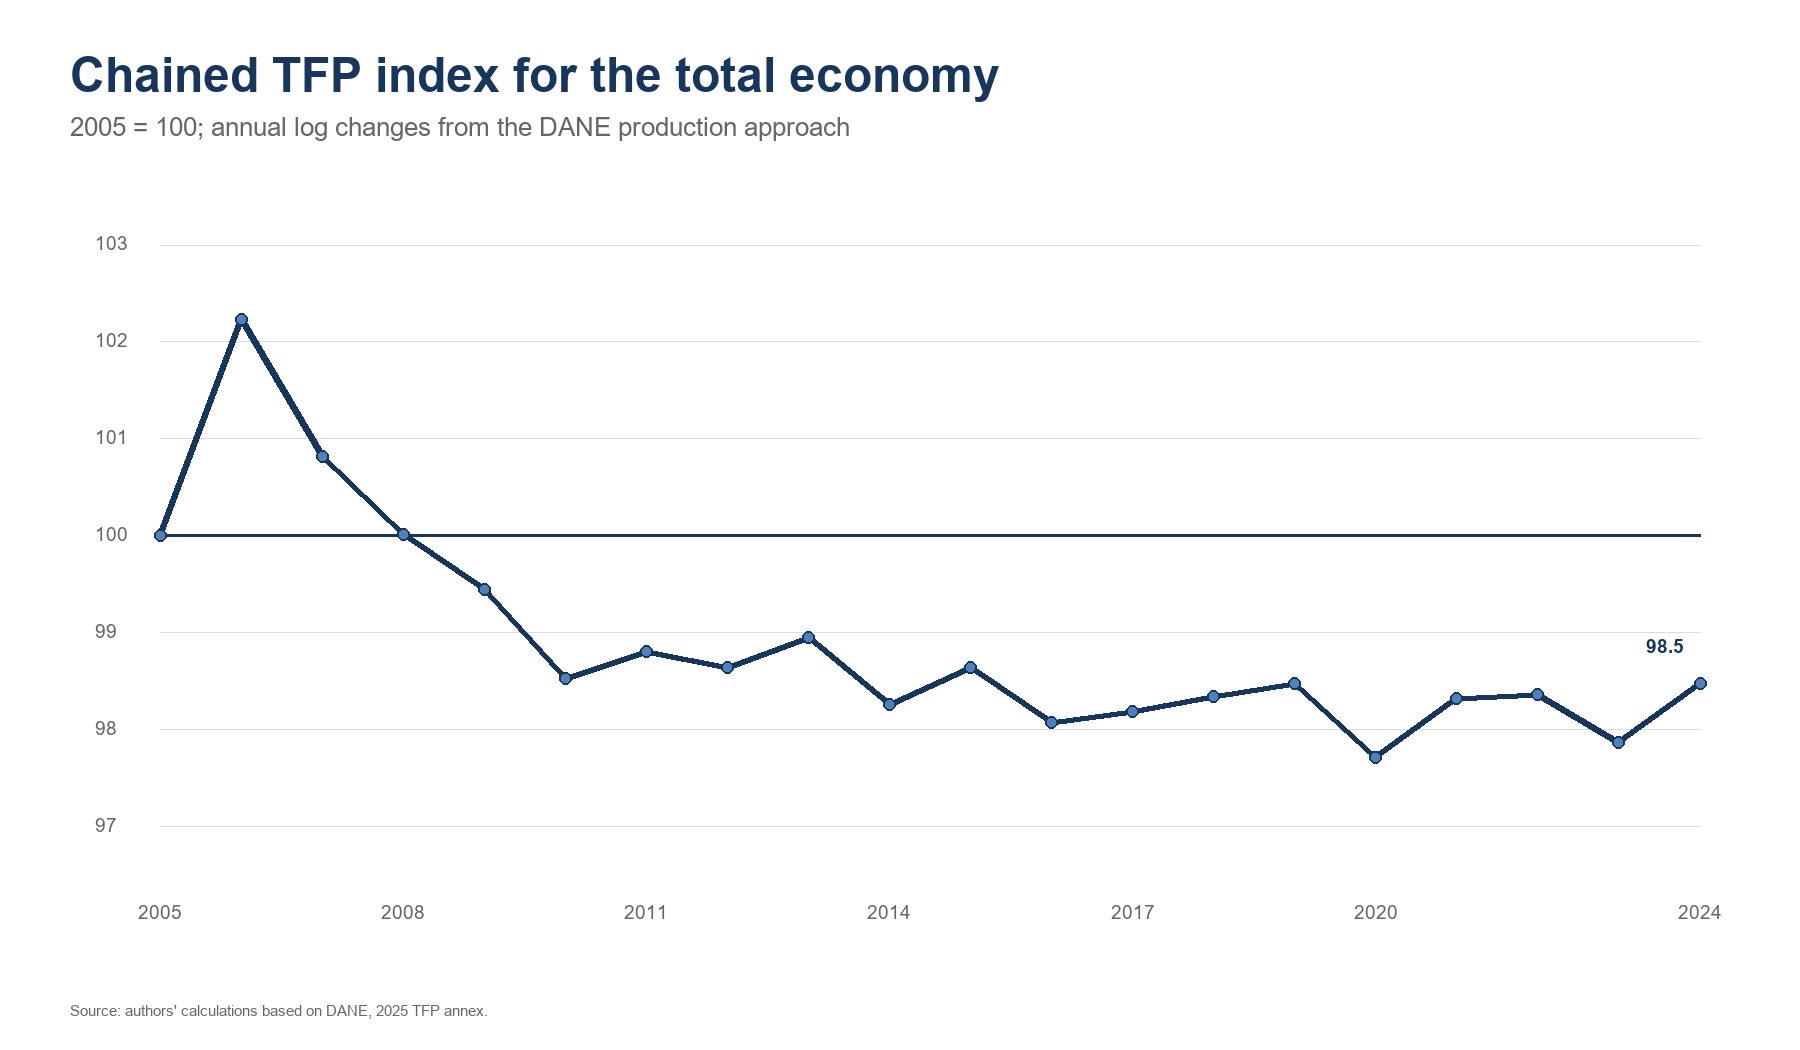
\includegraphics[width=0.93\textwidth]{paper_fig_ptf_total_index.png}
  \caption{Chained TFP index for the total economy, 2004--2024}
  \label{fig:paper_total_index}
\end{figure}

Most of the aggregate decline occurred before 2011. Aggregate TFP averaged $-0.235$ percent per year in 2005--2010. The subsequent averages were close to zero: 0.022 percent in 2011--2015, $-0.040$ in 2016--2019, and $-0.001$ in 2020--2024. The early deterioration stopped, but aggregate TFP did not enter a sustained growth path.

\subsection{Aggregate stagnation concealed sectoral paths moving in opposite directions}

Figure~\ref{fig:paper_heatmap} displays the 20 annual TFP growth rates that determine the long-run results. The activities are ranked from the lowest to the highest cumulative TFP growth, with the total economy shown in the final row. Mining recorded negative TFP growth in 17 of 20 years and manufacturing in 15. Agriculture and trade recorded positive TFP growth in 15 years; social services did so in 14.

\begin{figure}[H]
  \centering
  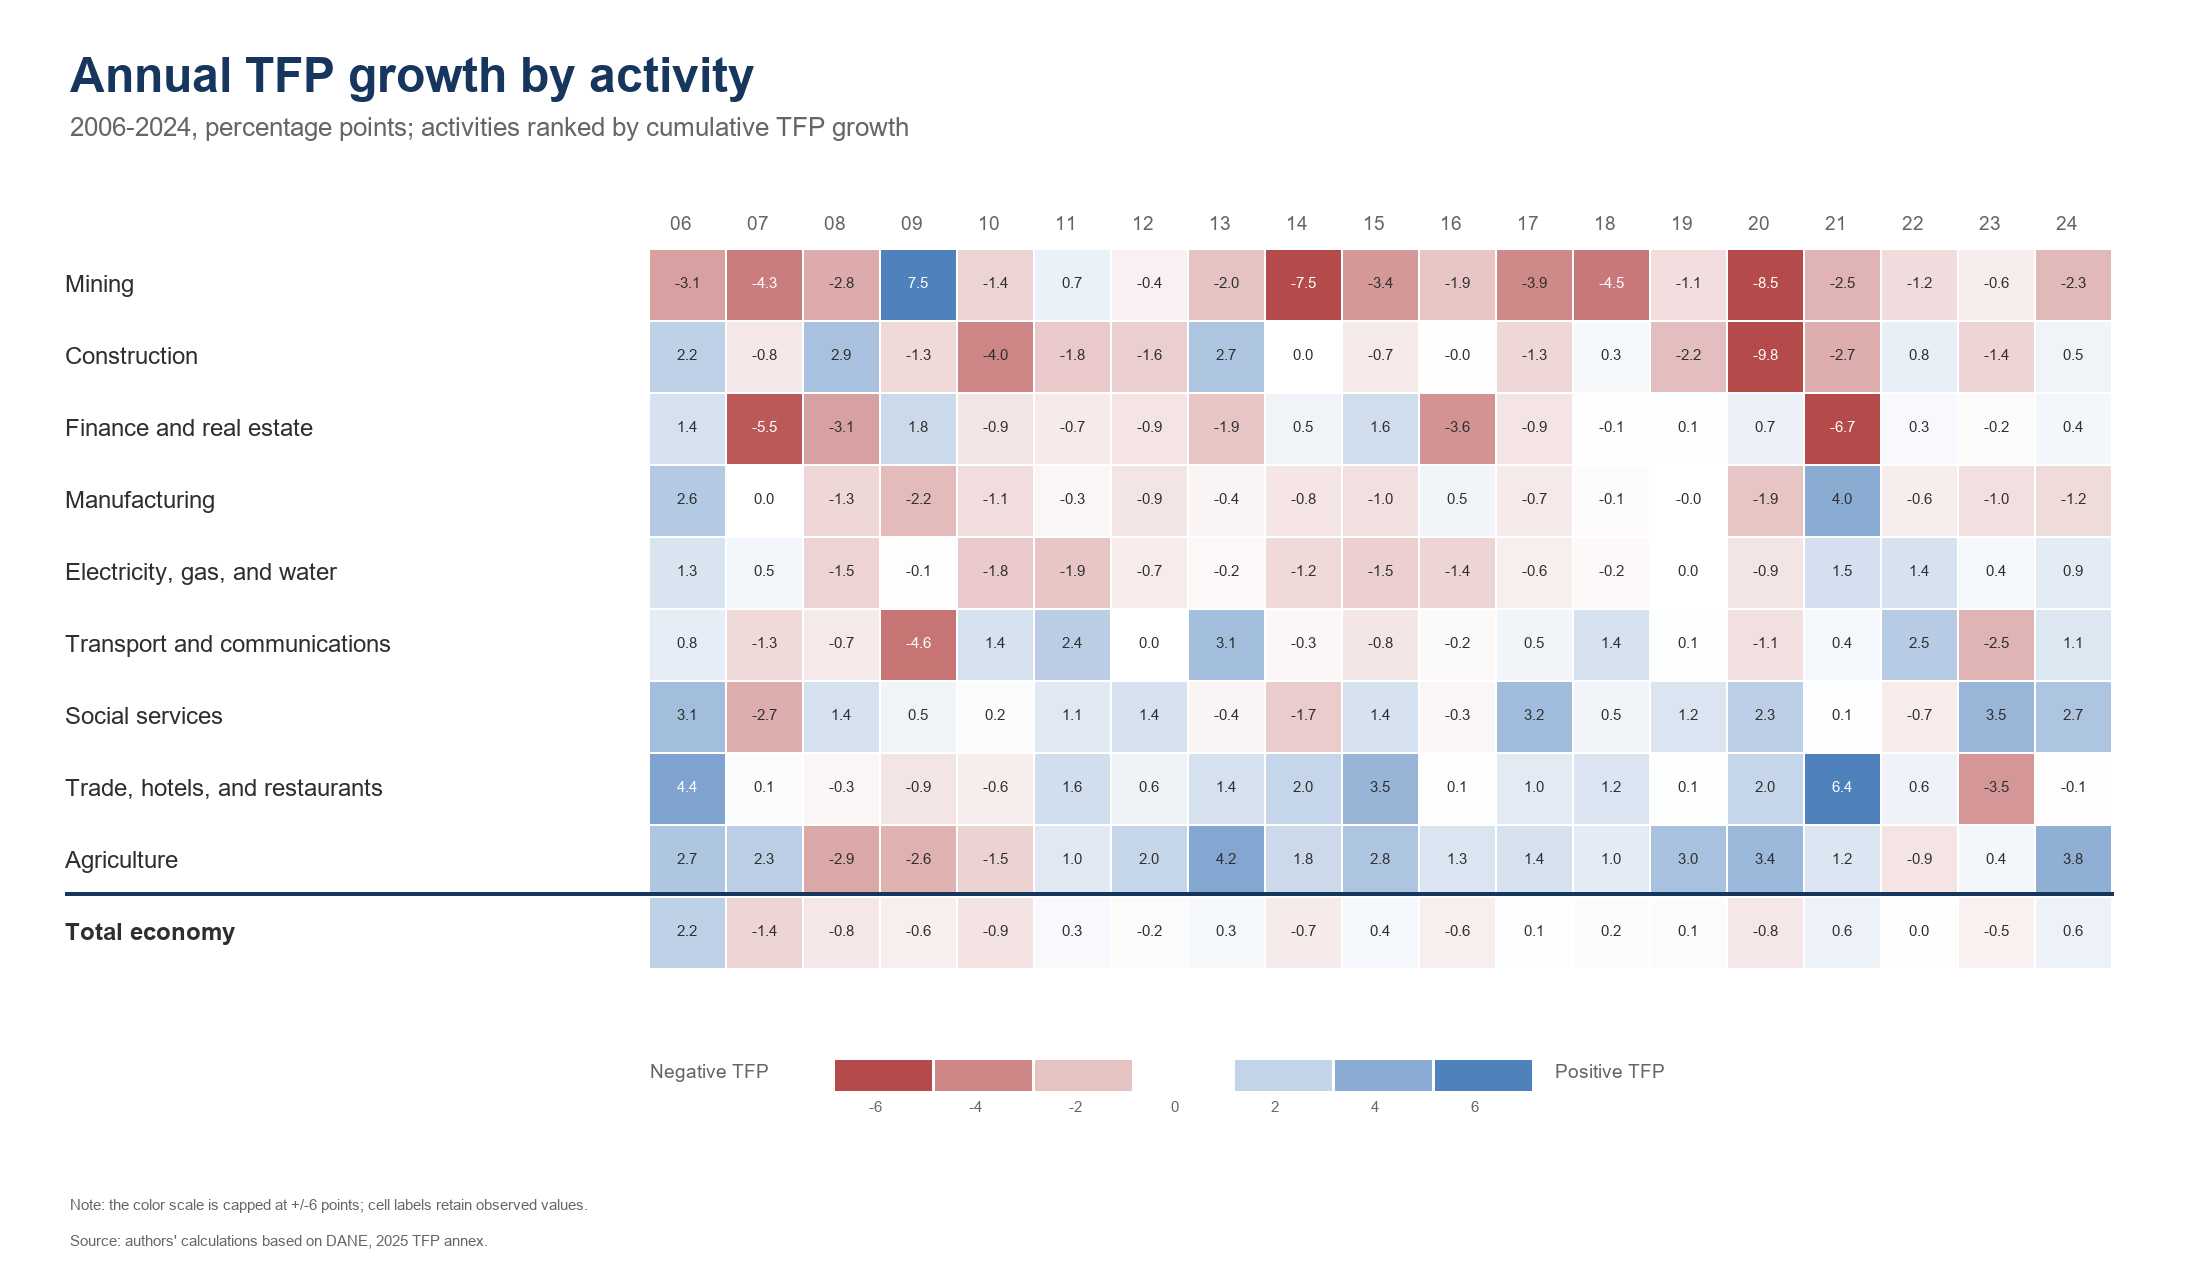
\includegraphics[width=\textwidth]{paper_fig_ptf_heatmap.png}
  \caption{Annual TFP growth for the total economy and nine activities, 2005--2024}
  \label{fig:paper_heatmap}
\end{figure}

The annual observations also show why long-run averages should not be interpreted as smooth trends. Construction TFP fell by 9.8 percentage points in 2020. Trade TFP increased by 6.4 points in 2021, while finance and real estate fell by 6.7 points. These changes affect the full-period averages, but the sign frequencies show that the strongest long-run results are not produced by a single year alone.

Figure~\ref{fig:paper_sector_performance} reports the cumulative and annualized measures. Trade had the highest cumulative TFP growth, 23.2 percent, equivalent to an annualized rate of 1.04 percent. Agriculture increased by 21.8 percent and social services by 14.2 percent. Mining had the largest decline, 32.1 percent, equivalent to an annualized rate of $-1.93$ percent. Finance and real estate lost 19.0 percent and construction 11.1 percent.

\begin{figure}[H]
  \centering
  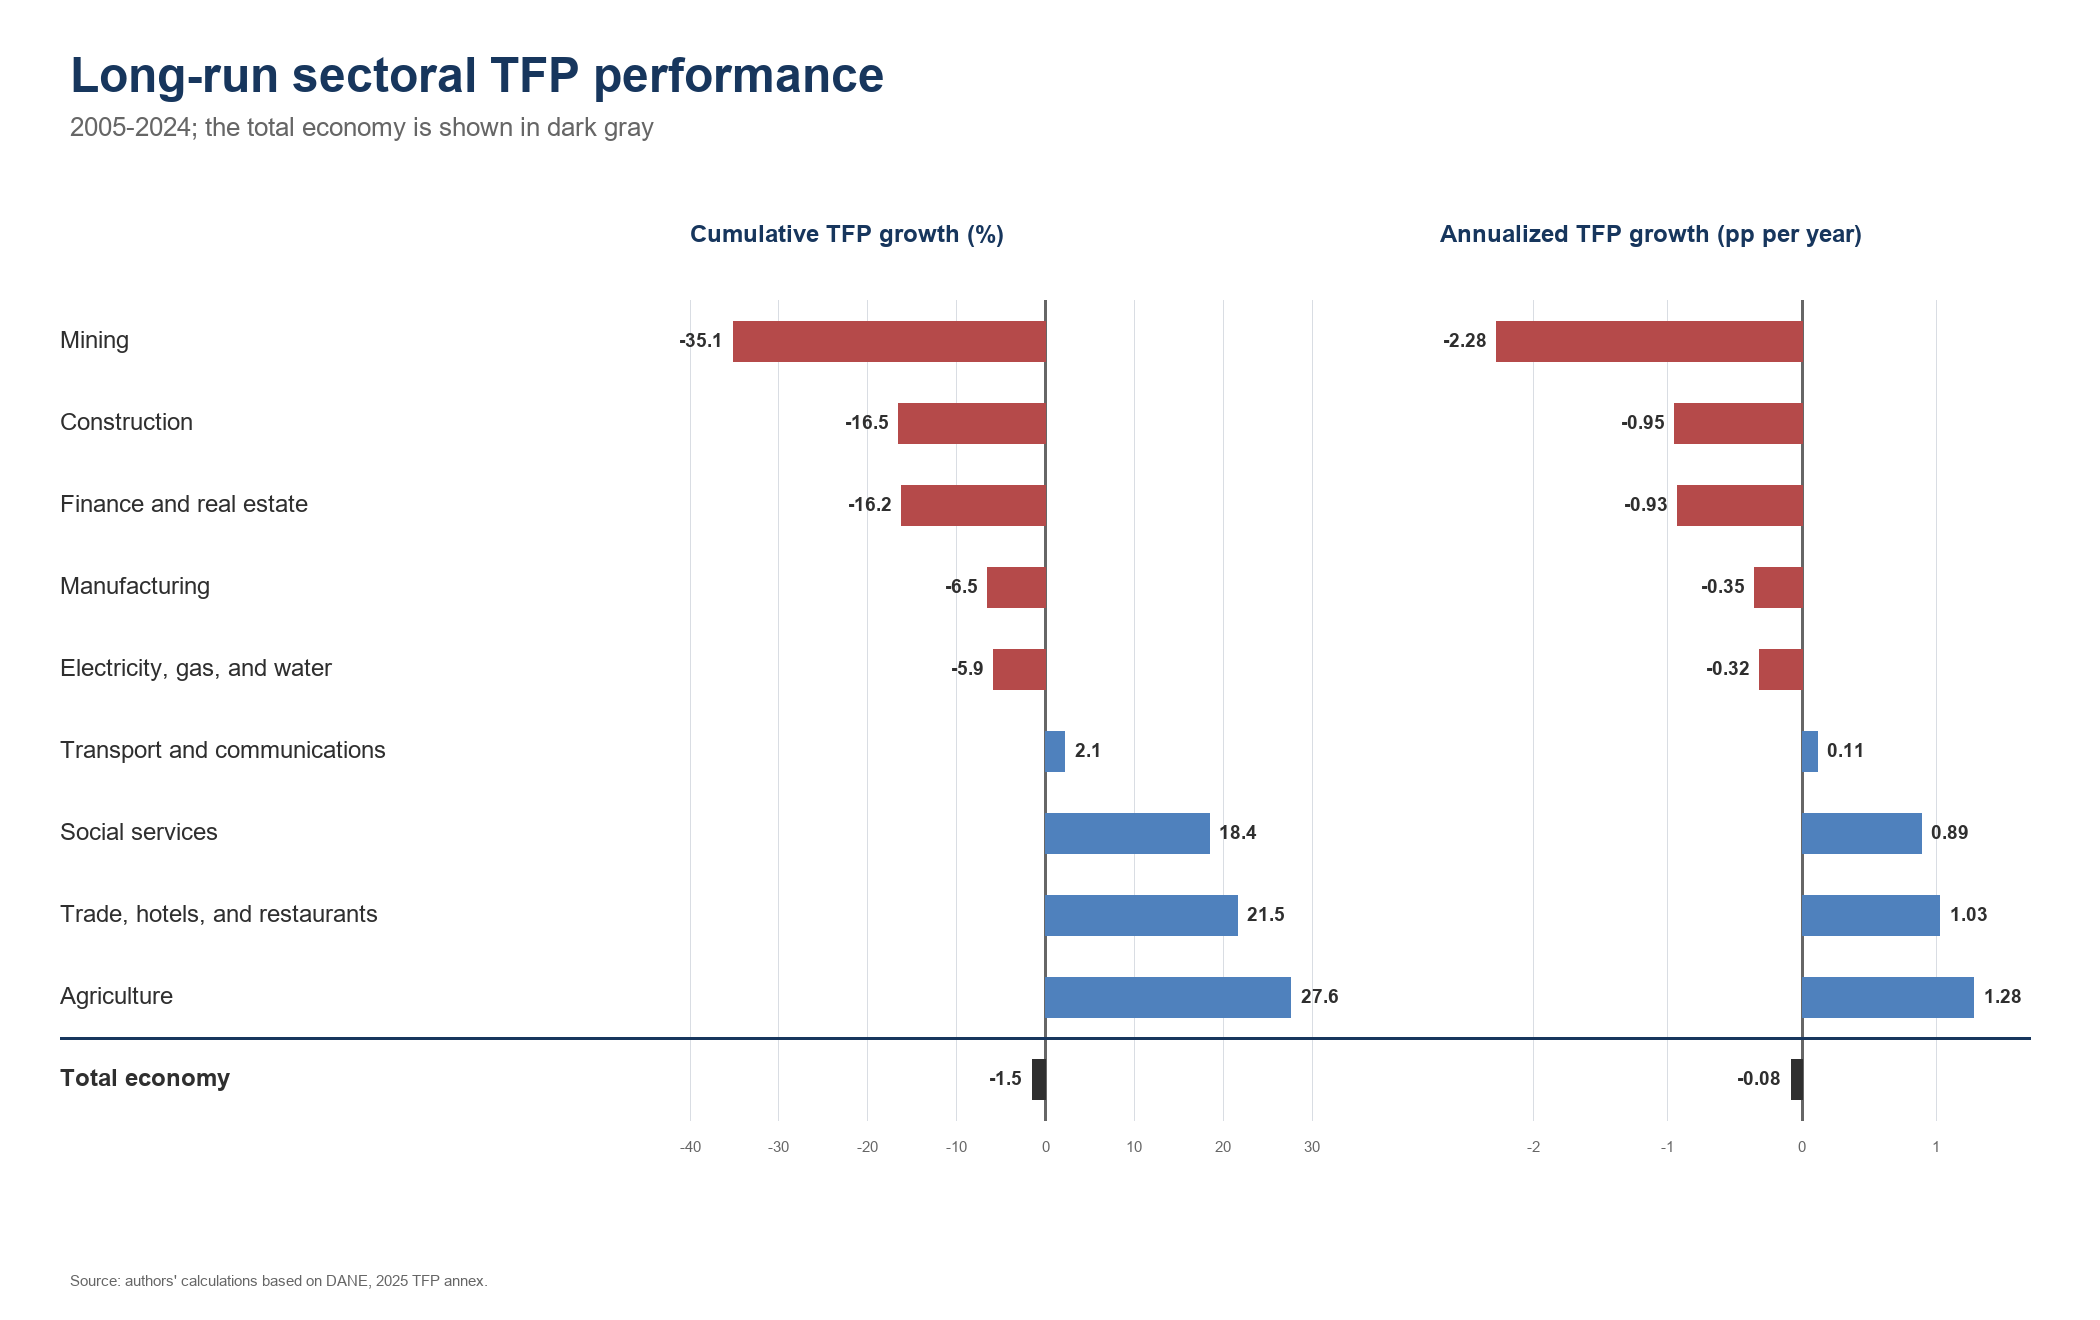
\includegraphics[width=\textwidth]{paper_fig_ptf_sector_performance.png}
  \caption{Cumulative TFP growth from 2004 to 2024 and annualized growth over 2005--2024}
  \label{fig:paper_sector_performance}
\end{figure}

\subsection{Positive and negative sectoral contributions nearly offset}

Sectoral TFP growth does not determine an activity's aggregate contribution on its own. The contribution also depends on its annual aggregation weight. Figure~\ref{fig:paper_contributions} and Table~\ref{tab:paper_long_run} report both dimensions. Four activities contributed 6.308 cumulative log points, or 0.315 percentage points per year. Five activities subtracted 7.770 cumulative log points, or 0.389 points per year. The net contribution was $-1.462$ log points, equivalent to the aggregate annualized TFP growth rate of $-0.073$ percent.

\begin{figure}[H]
  \centering
  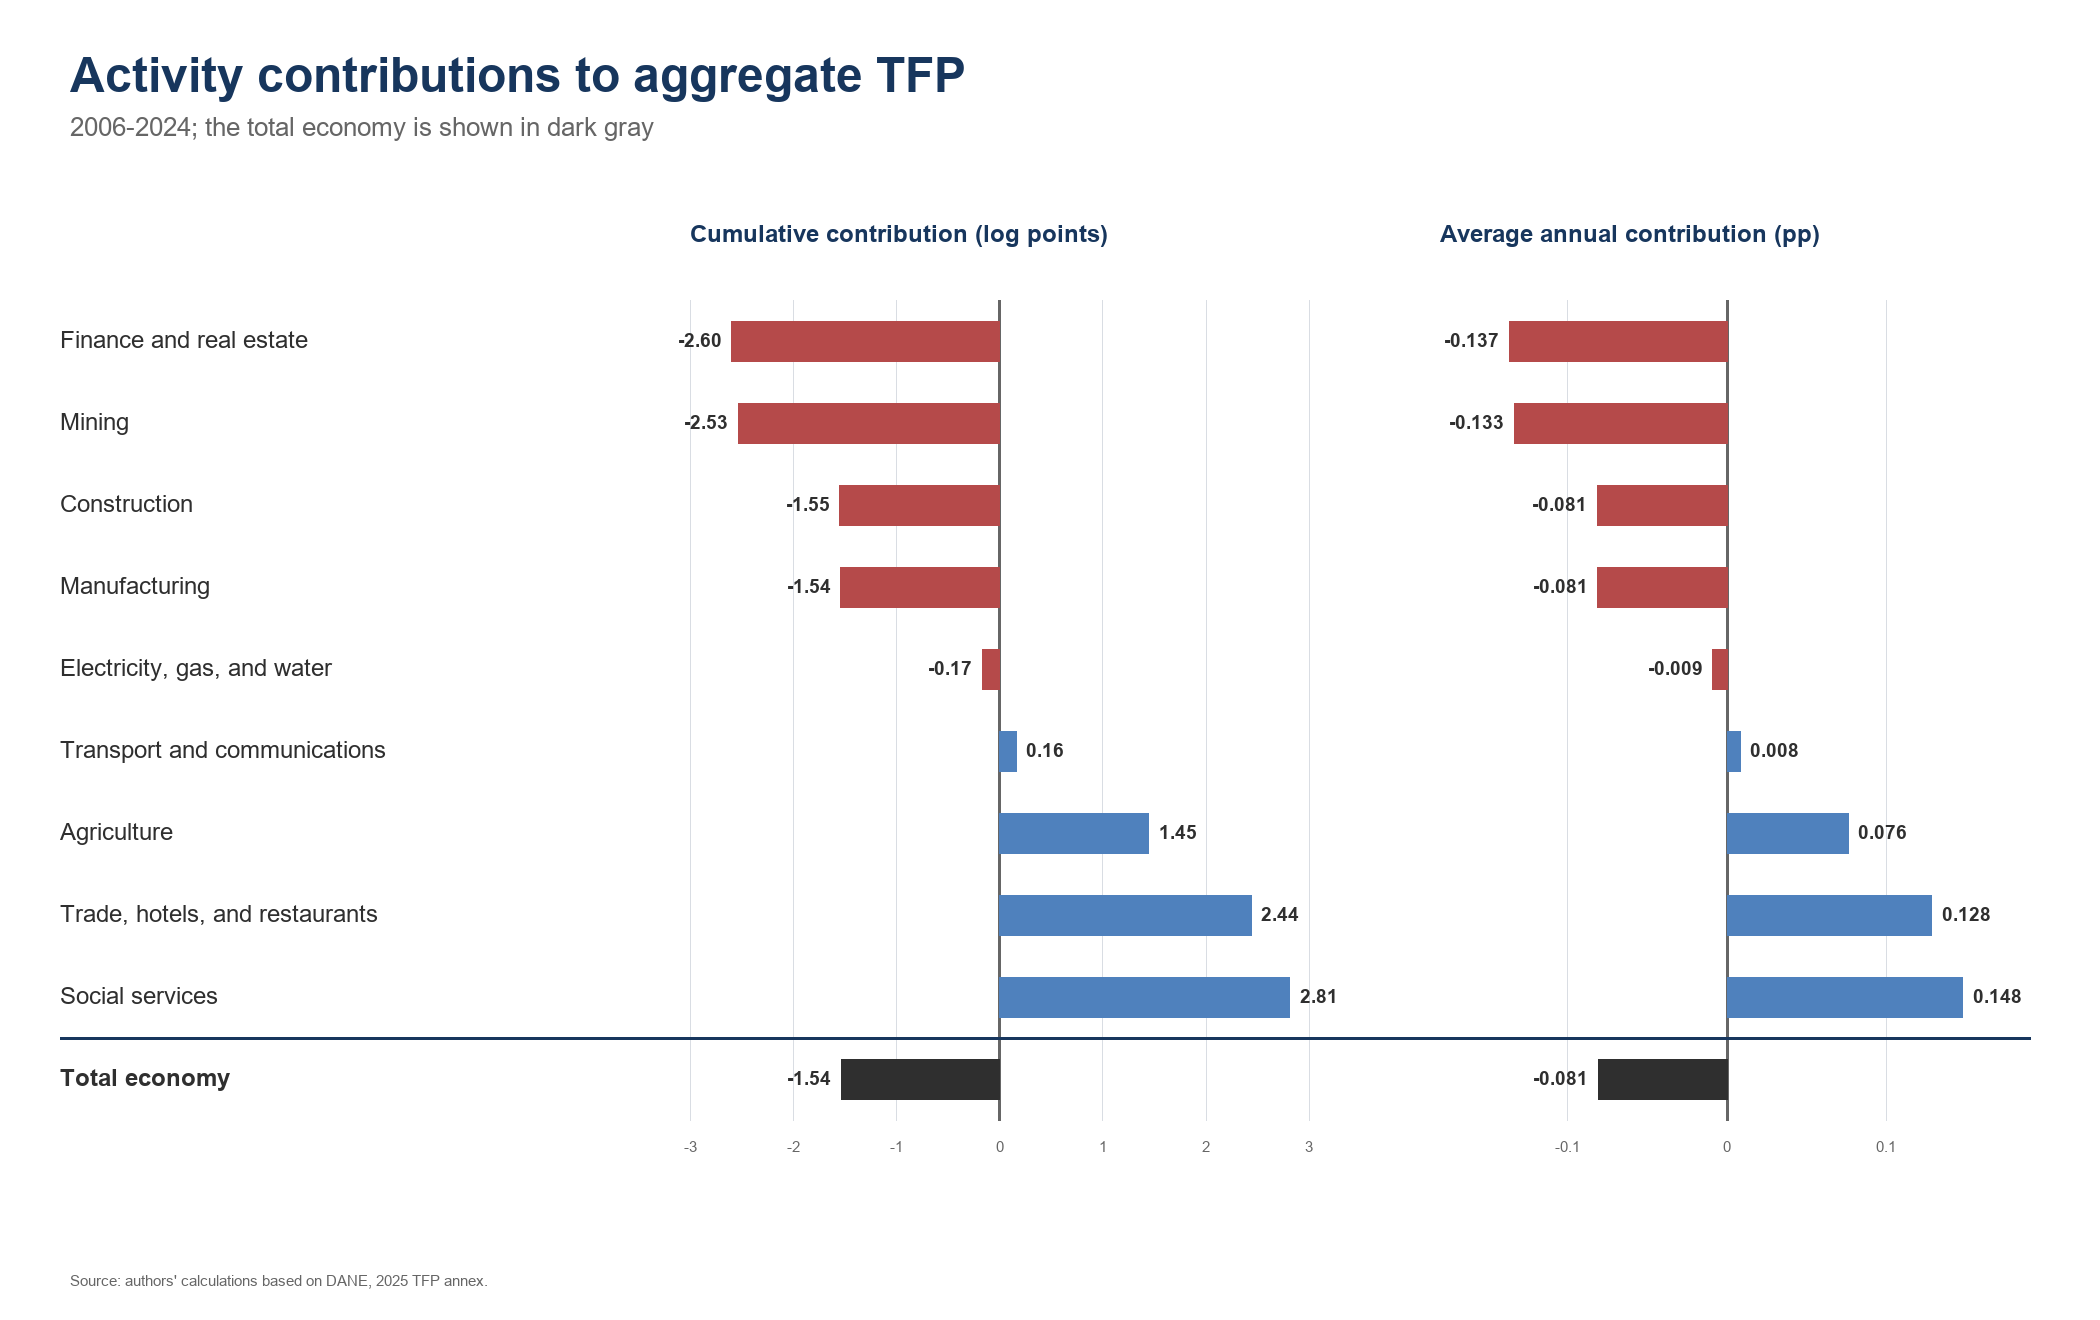
\includegraphics[width=\textwidth]{paper_fig_ptf_contributions.png}
  \caption{Activity contributions to aggregate TFP, 2005--2024}
  \label{fig:paper_contributions}
\end{figure}

\begin{table}[H]
\centering
\caption{Sectoral TFP performance and contribution to the total economy, 2005--2024}
\label{tab:paper_long_run}
\footnotesize
\setlength{\tabcolsep}{3pt}
\begin{tabular}{p{4.3cm}rrrr}
\toprule
Activity & Average weight & Cumulative TFP & Annualized TFP & Contribution \\
 & (\%) & growth, 2004--24 (\%) & growth (\%) & (pp per year) \\
\midrule
Trade, hotels, and restaurants & 12.98 & 23.17 & 1.04 & 0.130 \\
Social services & 16.05 & 14.16 & 0.66 & 0.112 \\
Agriculture & 6.11 & 21.84 & 0.99 & 0.056 \\
Transport and communications & 8.63 & 4.26 & 0.21 & 0.017 \\
Electricity, gas, and water & 3.42 & -5.53 & -0.28 & -0.008 \\
Construction & 8.64 & -11.06 & -0.59 & -0.054 \\
Manufacturing & 23.43 & -5.15 & -0.26 & -0.058 \\
Mining & 6.08 & -32.09 & -1.93 & -0.115 \\
Finance and real estate & 14.66 & -19.01 & -1.05 & -0.154 \\
\midrule
\textbf{Total economy} & \textbf{100.00} & \textbf{-1.45} & \textbf{-0.07} & \textbf{-0.073} \\
\bottomrule
\end{tabular}
\vspace{0.15cm}
\begin{minipage}{0.96\textwidth}
\footnotesize \textit{Notes:} Cumulative growth compares the 2024 chained index with 2004. Annualized TFP is the mean of the 20 annual log growth rates from 2005 through 2024. Sectoral cumulative and annualized TFP describe performance within each activity and do not add across activities. The contribution multiplies annual activity TFP by its annual weight before averaging; the nine contributions add to aggregate TFP. Figures may not add because of rounding.
\par\textit{Source:} Authors' calculations based on DANE, 2025 TFP annex.
\end{minipage}
\end{table}


Trade made the largest positive contribution, at 0.130 percentage points per year. Its average weight was 13.0 percent and its own TFP increased at an annualized rate of 1.04 percent. Social services contributed 0.112 points. Agriculture had a lower average weight of 6.1 percent, so its contribution was 0.056 points. Transport contributed 0.017 points.

Finance and real estate made the largest negative contribution, at $-0.154$ percentage points per year. Its own TFP fell at an annualized rate of 1.05 percent and its average weight was 14.7 percent. Mining subtracted 0.115 points. Its average weight was only 6.1 percent, but its own TFP decline was much larger at 1.93 percent per year.

Manufacturing and construction subtracted 0.058 and 0.054 percentage points per year, respectively. Manufacturing had the largest average weight, 23.4 percent, but its own TFP fell at an annualized rate of 0.26 percent. Construction had an average weight of 8.6 percent and a larger sectoral decline of 0.59 percent. These cases show why rankings based only on sectoral TFP growth do not identify the activities with the largest aggregate effect.

\subsection{A zero-TFP counterfactual raises production-account output growth}

Figure~\ref{fig:paper_counterfactual} shows the accounting counterfactual. Production-account output grew by 3.26 percent per year between 2005 and 2024. Setting annual TFP growth to zero in the four weakest activities raises the average to 3.59 percent. The difference is 0.331 percentage points per year.

\begin{figure}[H]
  \centering
  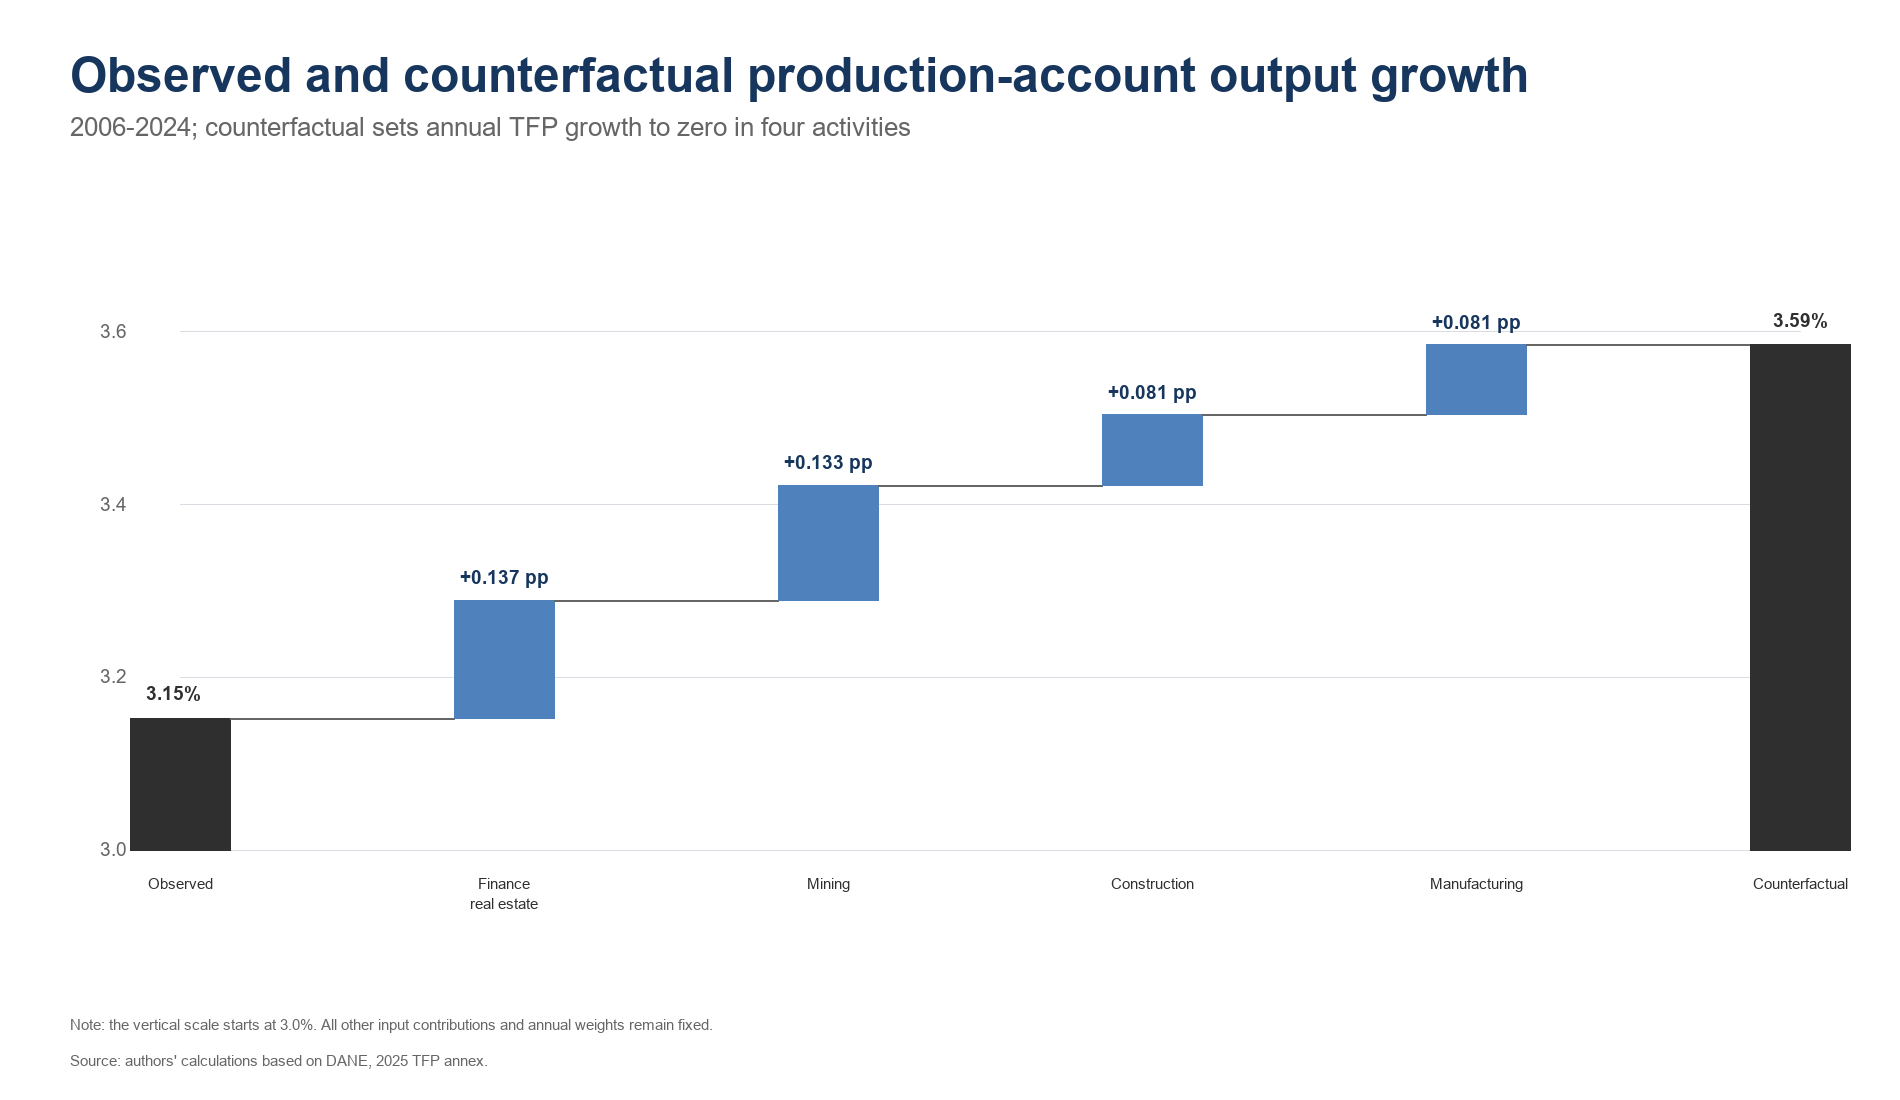
\includegraphics[width=0.95\textwidth]{paper_fig_ptf_counterfactual.png}
  \caption{Observed and counterfactual production-account output growth, 2005--2024}
  \label{fig:paper_counterfactual}
\end{figure}

Finance and real estate and mining account for 0.269 of the 0.331 additional points. Setting finance and real estate TFP growth to zero adds 0.154 points per year, and doing the same for mining adds 0.115. Construction adds 0.054 points and electricity, gas, and water adds 0.008. These changes equal the negative of their average TFP contributions because the exercise holds all other components fixed.

The counterfactual raises output growth in 15 of the 20 years. It lowers growth in 2005, 2006, 2009, 2022, and 2024 because the four selected activities made a positive joint TFP contribution in those years. Compounding the annual differences implies a production-account output level in 2024 that is 6.8 percent above the observed level.

This result should not be interpreted as a policy estimate. It shows the amount of observed growth associated with the negative TFP contributions under the KLEMS identity. It does not show that zero TFP growth was feasible, which intervention could have achieved it, or how factor use and relative prices would have responded.

\section{Discussion}

The aggregate result changes meaning once it is decomposed. Colombia's production-account TFP was nearly flat over 2005--2024, but this was not the common outcome of all activities. Social services, trade, agriculture, and transport made positive contributions that were almost fully offset by finance and real estate, mining, construction, manufacturing, and electricity. The relevant empirical question is therefore not only why aggregate TFP stagnated. It is also why productivity gains persisted in some activities while negative contributions remained large in others.

The results do not identify the mechanisms behind each activity path. Mining illustrates the limitation. Its output grew by 1.70 percent per year, but the measured input contributions exceeded that growth and produced TFP of $-2.28$ points. This pattern may reflect resource depletion, the composition of extraction, investment cycles, capacity utilization, regulation, or measurement. The data used here cannot distinguish among these explanations.

Finance and real estate present a different problem. The combined aggregate covers financial intermediation, real estate, and business and rental activities. Its negative contribution may therefore combine distinct subactivities. Output and price measurement are also difficult in financial and real-estate services. A useful extension would reconstruct the contribution at a finer level before assigning a common mechanism to the aggregate.

Manufacturing and construction show why both the sectoral change and the aggregation weight matter. Manufacturing had a moderate TFP decline but a large average weight. Construction had a sharper decline and a smaller weight. Their average aggregate contributions were almost identical. A policy diagnosis based only on the largest sectoral decline would miss manufacturing's aggregate relevance.

The counterfactual provides a scale for these negative contributions, not a policy target. Raising sectoral TFP requires changes in technology, organization, regulation, factor allocation, capacity use, or measurement, depending on the activity. A credible policy exercise must replace the zero-TFP benchmark with attainable sector-specific references and allow labor, capital, intermediate inputs, prices, and activity weights to respond.

The next empirical step should therefore be sector-specific. For manufacturing, the evidence should test the roles of technology adoption, management practices, exporting, and firm reallocation. For construction, it should distinguish project-cycle and capacity-utilization effects from persistent weaknesses in project management and production methods. For mining, it should separate resource and composition effects from investment and regulatory conditions. For finance and real estate, the first requirement is a more detailed statistical decomposition.

The analysis also has two general limitations. First, the period begins in 2005 because the sectoral production-account history in the annex is reported as annual changes rather than a longer published index. Second, the recovered weights are implicit in the DANE aggregation. Their exact reconciliation supports the contribution calculation, but the public annex does not expose the underlying nominal series used to construct them. Replication therefore validates the accounting system, not every stage of DANE's source-data construction.

\section{Conclusion}

Aggregate TFP did not grow in Colombia between 2005 and 2024. The chained index fell from 100 to 98.5, a cumulative decline of 1.5 percent and an annualized log change of $-0.081$ percentage points. Most of the decline occurred before 2011, but the subsequent improvement did not become sustained aggregate TFP growth.

The aggregate result was produced by large contributions of opposite signs. Social services, trade, agriculture, and transport contributed 0.361 percentage points per year. Finance and real estate, mining, construction, manufacturing, and electricity subtracted 0.441 points. Finance and real estate and mining made the largest negative contributions, while social services made the largest positive contribution.

The year-by-year aggregation is central to this conclusion. Cumulative sectoral TFP growth does not add across activities, and average weights applied to long-run sectoral growth do not reproduce the exact total when weights change over time. Recovering the annual weights and averaging annual contributions preserves the published aggregate identity.

The accounting counterfactual shows the scale of the negative contributions. If annual TFP growth in the four weakest activities had been zero, production-account output growth would have been 3.59 percent per year rather than 3.15 percent. The 0.43-point difference is economically meaningful, but it is not a causal estimate or a forecast of GDP. The result identifies where a more detailed diagnosis may have the highest aggregate payoff. It does not identify the policies that would produce those gains.


\appendix
\begin{landscape}
\begingroup
\small
\setlength{\tabcolsep}{4pt}
\begin{longtable}{p{4.4cm}rrrrrrr}
\caption{Average annual decomposition of output growth by activity, 2006--2024}
\label{tab:paper_growth_accounting}\\
\toprule
Activity & Output & Labor & Capital & Energy & Materials & Services & TFP \\
\midrule
\endfirsthead
\toprule
Activity & Output & Labor & Capital & Energy & Materials & Services & TFP \\
\midrule
\endhead
\textbf{Total economy} & \textbf{3.15} & \textbf{0.87} & \textbf{0.93} & \textbf{0.20} & \textbf{0.49} & \textbf{0.73} & \textbf{-0.08} \\
\midrule
Agriculture & 2.62 & -0.26 & 0.62 & 0.07 & 0.73 & 0.17 & 1.28 \\
Mining & 1.70 & 0.74 & 2.99 & 0.20 & 0.01 & 0.05 & -2.28 \\
Manufacturing & 1.92 & 0.19 & 0.77 & 0.27 & 0.90 & 0.14 & -0.35 \\
Electricity, gas, and water & 2.67 & 0.22 & 1.25 & 1.33 & 0.06 & 0.13 & -0.32 \\
Construction & 1.94 & 0.69 & 0.84 & 0.03 & 1.24 & 0.09 & -0.95 \\
Trade, hotels, and restaurants & 3.71 & 0.84 & 0.16 & 0.10 & 0.47 & 1.11 & 1.03 \\
Transport and communications & 4.05 & 1.20 & 0.70 & 0.59 & 0.11 & 1.33 & 0.11 \\
Finance and real estate & 3.90 & 1.70 & 2.04 & 0.01 & 0.05 & 1.03 & -0.93 \\
Social services & 4.59 & 1.68 & 0.07 & 0.04 & 0.31 & 1.60 & 0.89 \\
\bottomrule
\multicolumn{8}{p{15.9cm}}{\footnotesize \textit{Notes:} Values are average annual percentage-point contributions, except output, which is the average annual log growth rate. The 19 observations from 2006 to 2024 connect the levels in 2005 and 2024. The total-economy row is the DANE published aggregate, not a simple sum or average of the activity rows. Components may not add exactly because of rounding.}\\
\multicolumn{8}{l}{\footnotesize \textit{Source:} Authors' calculations based on DANE, 2025 TFP annex.}\\
\end{longtable}
\endgroup
\end{landscape}


\section{Contributions by Subperiod}

\begin{table}[H]
\centering
\caption{Activity contributions to aggregate TFP by subperiod}
\label{tab:paper_subperiods}
\footnotesize
\setlength{\tabcolsep}{3pt}
\begin{tabular}{p{4.6cm}rrrrr}
\toprule
Activity & 2005--10 & 2011--15 & 2016--19 & 2020--24 & 2005--24 \\
\midrule
Agriculture & -0.069 & 0.122 & 0.094 & 0.110 & 0.056 \\
Mining & 0.009 & -0.193 & -0.155 & -0.153 & -0.115 \\
Manufacturing & -0.022 & -0.157 & -0.021 & -0.031 & -0.058 \\
Electricity, gas, and water & -0.006 & -0.035 & -0.018 & 0.026 & -0.008 \\
Construction & 0.059 & -0.022 & -0.078 & -0.202 & -0.054 \\
Trade, hotels, and restaurants & 0.085 & 0.216 & 0.077 & 0.140 & 0.130 \\
Transport and communications & -0.036 & 0.076 & 0.038 & 0.005 & 0.017 \\
Finance and real estate & -0.224 & -0.038 & -0.169 & -0.173 & -0.154 \\
Social services & -0.030 & 0.054 & 0.192 & 0.276 & 0.112 \\
\midrule
\textbf{Total economy} & \textbf{-0.235} & \textbf{0.022} & \textbf{-0.040} & \textbf{-0.001} & \textbf{-0.073} \\
\bottomrule
\end{tabular}
\vspace{0.15cm}
\begin{minipage}{0.96\textwidth}
\footnotesize \textit{Notes:} Average annual percentage-point contributions. Each activity entry is the subperiod mean of annual TFP multiplied by the annual aggregation weight. Subperiods have different lengths.
\par\textit{Source:} Authors' calculations based on DANE, 2025 TFP annex.
\end{minipage}
\end{table}


\section{Activity Coverage}

\small
\begin{longtable}{p{4.0cm}p{10.5cm}}
\caption{Correspondence between KLEMS aggregates and CIIU activities}
\label{tab:paper_sector_mapping}\\
\toprule
Activity aggregate & Included CIIU activities \\
\midrule
\endfirsthead
\toprule
Activity aggregate & Included CIIU activities \\
\midrule
\endhead
Agriculture &
\textbf{Section A:} agriculture, livestock, hunting, and forestry.
\textbf{Section B:} fishing. \\
\addlinespace
Mining &
\textbf{Section C:} mining and quarrying. \\
\addlinespace
Manufacturing &
\textbf{Section D:} manufacturing, including food and beverages; tobacco;
textiles and apparel; leather and footwear; wood; paper and printing;
petroleum refining; chemicals; rubber and plastics; non-metallic mineral
products; metals; machinery and equipment; electrical, electronic, and
transport equipment; and other manufacturing. \\
\addlinespace
Electricity, gas, and water &
\textbf{Section E:} electricity, gas, and water supply. \\
\addlinespace
Construction &
\textbf{Section F:} construction. \\
\addlinespace
Trade, hotels, and restaurants &
\textbf{Section G:} wholesale and retail trade; repair of motor vehicles,
motorcycles, personal effects, and household goods.
\textbf{Section H:} hotels and restaurants. \\
\addlinespace
Transport and communications &
\textbf{Section I:} transport, storage, and communications. \\
\addlinespace
Finance and real estate &
\textbf{Section J:} financial intermediation.
\textbf{Section K:} real estate, renting, and business activities. \\
\addlinespace
Social services &
\textbf{Section L:} public administration and defense; compulsory social security.
\textbf{Section M:} education.
\textbf{Section N:} health and social work.
\textbf{Section O:} other community, social, and personal service activities.
\textbf{Section P:} private households with employed persons and undifferentiated
production activities of private households.
\textbf{Section Q:} extraterritorial organizations and bodies. \\
\bottomrule
\multicolumn{2}{p{14.4cm}}{\footnotesize \textit{Notes:} The table documents
the correspondence between the nine aggregates in the DANE annex and the
CIIU Rev. 3/3.1 sections adapted for Colombia. Labels may vary across revisions
without changing the KLEMS aggregate used by DANE.}\\
\multicolumn{2}{l}{\footnotesize \textit{Source:} DANE, CIIU Rev. 3 and Rev. 3.1 A.C.; 2025 TFP annex.}\\
\end{longtable}
\normalsize



\section*{Data and Code Availability}

The DANE source annex, processed data, replication programs, figures, and table sources are available at:

\url{https://github.com/oliverpardo1979/informe_ptf}.

\noindent The original DANE annex is redistributed in the repository for reproducibility. Users should consult DANE for the official release and any subsequent revisions.

\bibliographystyle{apalike}
\small
\bibliography{Paper/references}

\end{document}
